\documentclass[10pt,twocolumn,letterpaper]{article}

\usepackage[labelfont=bf]{caption}
\usepackage[table]{xcolor}
\usepackage{graphicx}
\usepackage{multirow}
\usepackage{amsfonts}
\usepackage{amssymb}
\usepackage[tbtags]{amsmath}
\usepackage[a4paper,margin=4cm]{geometry}
\usepackage{lastpage}
\usepackage{fancyhdr}
\usepackage[round]{natbib}
\usepackage{listings}
\usepackage{color}
\usepackage[title]{appendix}
\usepackage{bm}
\usepackage{textcomp}
\usepackage{mathtools}
\usepackage{tabularx}
\usepackage{booktabs}
\usepackage{ragged2e}
\usepackage{float}
\usepackage{enumitem}
\usepackage{tabularx}
\usepackage{tikz}
\usetikzlibrary{fit, shapes.misc, positioning, arrows.meta, calc}

\bibliographystyle{plainnat}
\def\sumin{\sum_{i=1}^{n}}
\def\bhline{\noalign{\hrule height 1pt}}

\DeclarePairedDelimiter\abs{\lvert}{\rvert}

%table
\definecolor{faintgrey}{RGB}{242, 242, 242}
\def\evenrow{\rowcolor{faintgrey}}
\captionsetup[table]{skip=0pt}
\newcolumntype{L}{>{\raggedright\arraybackslash}X}

%notations
\def\nodedistance{0.4cm}
\definecolor{fc}{RGB}{251, 227, 214}
\definecolor{fc-relu}{RGB}{246, 198, 173}
\definecolor{input}{RGB}{97, 203, 244}

\tikzstyle{arrow} = [gray, -{Triangle[angle=45:1pt 3]}, line width=1.5pt]
\tikzstyle{thin-arrow} = [gray, -{Straight Barb[angle'=60,scale=2]}, line width=0.8pt]
\tikzstyle{connector} = [gray, -, >=stealth, line width=1.5pt]

\newcommand{\unitw}[2]{w_{#2}^{(#1)}}
\newcommand{\tikzlayernode}[1]{\node[
  draw=none, rounded rectangle, minimum width=1cm, minimum height=0.43cm, fill=#1, inner sep=0,
  font=\fontsize{8pt}{8pt}\selectfont
]}
\newcommand{\tikzinputnode}[1]{\node[
  draw=none, circle, minimum height=0.43cm, fill=#1, inner sep=0, font=\fontsize{8pt}{8pt}\selectfont
]}

\newcommand{\nnlayer}[2]{\begin{tikzpicture}[baseline=-0.1cm]
  \tikzlayernode{#1}{#2};
\end{tikzpicture}}

\newcommand{\nninput}[2]{\begin{tikzpicture}[baseline=-0.1cm]
  \tikzinputnode{#1}{#2};
\end{tikzpicture}}

%architectures
\newcommand{\architecturea}[1]{
  \begin{tikzpicture}[node distance=\nodedistance, baseline=#1]
    % nodes
    \tikzinputnode{input}   at (0, 0)           (input)   {};
    \tikzlayernode{fc}      [right = of input]  (output)  {10};

    % arrows
    \draw[arrow]  (input) -- (output);
  \end{tikzpicture}
}
\newcommand{\architectureb}[1]{
  \begin{tikzpicture}[node distance=\nodedistance, baseline=#1]
    % nodes
    \tikzinputnode{input}   at (0, 0)           (input)   {};
    \tikzlayernode{fc-relu} [right = of input]  (1)       {512};
    \tikzlayernode{fc-relu} [right = of 1]      (2)       {256};
    \tikzlayernode{fc}      [right = of 2]      (output)  {10};

    % arrows
    \draw[connector]  (input) -- (1);
    \draw[connector]  (1)     -- (2);
    \draw[arrow]      (2)     -- (output);
  \end{tikzpicture}
}
\newcommand{\architecturec}[1]{
  \begin{tikzpicture}[node distance=\nodedistance, baseline=#1]
    % nodes
    \tikzinputnode{input}   at (0, 0)           (input)   {};
    \tikzlayernode{fc-relu} [right = of input]  (1)       {1024};
    \tikzlayernode{fc-relu} [right = of 1]      (2)       {512};
    \tikzlayernode{fc}      [right = of 2]      (output)  {10};

    % arrows
    \draw[connector]  (input) -- (1);
    \draw[connector]  (1)     -- (2);
    \draw[arrow]      (2)     -- (output);
  \end{tikzpicture}
}
\newcommand{\architectured}[1]{
  \begin{tikzpicture}[node distance=\nodedistance, baseline=#1]
    % nodes
    \tikzinputnode{input}   at (0, 0)           (input)   {};
    \tikzlayernode{fc-relu} [right = of input]  (1)       {2048};
    \tikzlayernode{fc-relu} [right = of 1]      (2)       {1024};
    \tikzlayernode{fc}      [right = of 2]      (output)  {10};

    % arrows
    \draw[connector]  (input) -- (1);
    \draw[connector]  (1)     -- (2);
    \draw[arrow]      (2)     -- (output);
  \end{tikzpicture}
}
\newcommand{\architecturee}[1]{
  \begin{tikzpicture}[node distance=\nodedistance, baseline=#1]
    % nodes
    \tikzinputnode{input}   at (0, 0)           (input)   {};
    \tikzlayernode{fc-relu} [right = of input]  (1)       {4096};
    \tikzlayernode{fc-relu} [right = of 1]      (2)       {2048};
    \tikzlayernode{fc}      [right = of 2]      (output)  {10};

    % arrows
    \draw[connector]  (input) -- (1);
    \draw[connector]  (1)     -- (2);
    \draw[arrow]      (2)     -- (output);
  \end{tikzpicture}
}

% Include other packages here, before hyperref.

% If you comment hyperref and then uncomment it, you should delete
% egpaper.aux before re-running latex.  (Or just hit 'q' on the first latex
% run, let it finish, and you should be clear).
\usepackage[breaklinks=true,bookmarks=false]{hyperref}

\def\httilde{\mbox{\tt\raisebox{-.5ex}{\symbol{126}}}}

% Pages are numbered in submission mode, and unnumbered in camera-ready
%\ifcvprfinal\pagestyle{empty}\fi
%\setcounter{page}{4321}
\begin{document}

%%%%%%%%% TITLE
\title{Assessment 2: CNNs for Image Classification}

\author{Wasin Pipattungsakul \\
The University of Adelaide \\
{\tt\small wasin.pipattungsakul@adelaide.edu.au}
}

\maketitle
%\thispagestyle{empty}

%%%%%%%%% ABSTRACT
\begin{abstract}
  This work investigates the performance of convolutional neural network models, VGG16, VGG19, and ResNet50, on
  the CIFAR-10 dataset. These base models were connected with 5 different architectures and 2 learning rates
  were to observe the effect of additional hidden layers. ResNet50 showed the best performance on the validation
  and test sets with a certain configuration.
\end{abstract}

%%%%%%%%% BODY TEXT
\section{Introduction}

In this work, the performance of convolutional neural network models, VGG16, VGG19, and ResNet50, are compared
on the CIFAR-10 dataset \citep{data}. Transfer learning with several configurations were conducted on the
pretrained models to learn the target classes in the CIFAR-10 dataset. The

%-------------------------------------------------------------------------
\subsection{The CIFAR-10 Dataset}

According to \citet{data}, the CIFAR-10 dataset is part of the 80 million tiny images dataset. There are 60,000
32x32 colour images in the dataset. The images are classified into 10 mutually exclusive classes with their
corresponding numerical label below.
\begin{itemize}
  \item 0: airplane,
  \item 1: automobile,
  \item 2: bird,
  \item 3: cat,
  \item 4: deer,
  \item 5: dog,
  \item 6: frog,
  \item 7: horse,
  \item 8: ship, and
  \item 9: truck.
\end{itemize}

The Python version of the dataset was used for this work. The images are stored in a 2 dimensional (2D)
\href{https://numpy.org/}{numpy} array. Each record in the array (first dimension) contains 3,072 integers
(second dimension) which denote red, green, and blue channels in the first 1,024, second 1,024, and last 1,024
values, respectively.

The labels are stored in a list of integers in the range of 0 to 9, inclusively, with the meaning of the labels
explained above.

%-------------------------------------------------------------------------
\subsection{VGG16 \& VGG19}

The VGG models were submitted to the ILSVRC-2014 competition by a "VGG" team \citep{vgg}. VGG16 consists of 13
convolutional layers and 3 fully connected layers while VGG19 consists of 16 convolutional layers and 3 fully
connected layers. The models were trained on more than 1.3 million images with 1,000 classes. The validation and
testing were performed on 50,000 images and 100,000 images, respectively.

%-------------------------------------------------------------------------
\subsection{ResNet50}

ResNet models were developed by a team from Microsoft as their foundations for the submissions to ILSVRC \& COCO
2015 competitions \citep{resnet50}. ResNet50 consists of 49 convolutional layers with extra features and 1 fully
connected layer.

%------------------------------------------------------------------------
\section{Methods}

%-------------------------------------------------------------------------
\subsection{Data}

The CIFAR-10 dataset was split into:
\begin{itemize}
  \item Training set: 40,000 records
  \item Validation set: 10,000 records
  \item Test set: 10,000 records
\end{itemize}
Then, each record (an array of 3,072 integers) was reshaped to a 3D array (32x32x3) to represent the pixels of
an image before being transformed from RGB to BGR and zero-centered to be compatible with each model.

%-------------------------------------------------------------------------
\subsection{Learning Architecture Notations}

\begin{table}[!ht]
  \centering
  \caption{Symbols of layers in learning neural network architectures}
  \label{tab:notations}
  \begin{tabularx}{\columnwidth}{cL}
    \rowcolor{lightgray}
    \bf Symbol            & \bf Description \\
    \hline
    \nnlayer{fc}{n}       & A fully connected layer with n units and softmax activation \\
    \evenrow
    \nnlayer{fc-relu}{n}  & A fully connected layer with n units and ReLU activation \\
    \nninput{input}{}     & An flattened output from pretrained model
  \end{tabularx}
\end{table}
Throughout the report, the symbols in table \ref{tab:notations} are used in figures to describe learning
architectures.
\begin{figure}[!ht]
  \centering
  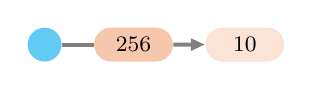
\begin{tikzpicture}[node distance=\nodedistance]
    % nodes
    \tikzinputnode{input}   at (0, 0)           (input)   {};
    \tikzlayernode{fc-relu} [right = of input]  (1)       {256};
    \tikzlayernode{fc}      [right = of 1]      (output)  {10};

    % arrows
    \draw[connector]  (input) -- (1);
    \draw[arrow]      (1)     -- (output);
  \end{tikzpicture}
  \caption{An example of neural network architecture with the symbols defined in table \ref{tab:notations}}
  \label{fig:example-architecture}
\end{figure}

For example, figure \ref{fig:example-architecture} illustrates a learning architecture with
\begin{enumerate}
  \item an output from the pretrained layers as an input,
  \item a fully connected layer with 256 units and ReLU activation as the only hidden layer,
  \item a fully connected layer with 10 units (classes) as an output.
\end{enumerate}

%-------------------------------------------------------------------------
\subsection{Model Training}

All models were developed in Python TensorFlow with model workloads executed on a GPU and a random seed of 112.
For each model, in all convolutional layers, the pretrained weights were loaded and not further trained. Then, a
few architectures with fully connected layers were connected to the pretrained layers and trained with the
training set. All models were tuned with the hyperparameters in table \ref{tab:hyperparameters}.
\begin{table}[!ht]
  \centering
  \caption{Hyperparameters used to train and tune the models}
  \label{tab:hyperparameters}
  \begin{tabularx}{\columnwidth}{Lp{89pt}}
    \rowcolor{lightgray}
    \bf Parameter         & \bf Value(s) \\
    \bhline
    Number of iterations  & 10,000, stopping after no improvement in 20 iterations on the validation set \\
    \evenrow
    Learning rate         & [0.0001, 0.001] \\
    Batch size            & 4096 \\
    \evenrow
    Learning architecture & 5 architectures (see Appendix A)
  \end{tabularx}
\end{table}
The best configuration for each model was then chosen based on the accuracy on the validation set following the
formulas
\begin{align}
  1_{\{a,b\}} = \left\{
    \begin{array}{ll}
      1,  & a=b \\
      0,  & \text{otherwise}
    \end{array}
  \right. \\
  \text{accuracy} = 1 - \frac{\sumin1_{\{y_i, \hat{y}_i\}}}{n}
\end{align}
where $y_i$ is the target label and $\hat{y}_i$ is the prediction of an $i$th record in the validation set.

%table for best performance
\input{./best-performance.tex}

%-------------------------------------------------------------------------
\section{Code}

The implementation can be found \href{https://github.com/wvjgsuhp/deep-learning-fundamentals-ass-2}{here}.

%-------------------------------------------------------------------------
\section{Results}

%-------------------------------------------------------------------------
\subsection{Overall Accuracy}

Figure \ref{fig:overall-performance} shows that ResNet50 has a narrow range of accuracies (0.64 - 0.67) on the
validation set across different configurations. It also provides the best overall accuracy among all models and
all configurations. VGG16 and VGG19 share roughly the same wide range of accuracies (0.57 - 0.66).
\begin{figure}[!ht]
  \centering
  \includegraphics[width=\columnwidth]{../assets/violin_plot.pdf}
  \caption{Overall accuracies of models on the validation set}
  \label{fig:overall-performance}
\end{figure}

%-------------------------------------------------------------------------
\subsection{Best Performance}

From table \ref{tab:model-performance}, the best configuration for ResNet50 yields a validation accuracy of 0.67
with a learning rate of 0.001 and 2 fully connected layers with ReLU activation before the output layer with
softmax activation. On the other hand, the best configurations for VGG16 and VGG19 require no additional hidden
layers between the output layer and the output from the pretrained layers. Thus, ResNet50 model would be chosen
for a real world application with the highest accuracy on the validation set. As an observation, it also yields
the best accuracy on the test set (0.666).

%-------------------------------------------------------------------------
\subsection{Performance with Different Architectures}

The performances on validation set of ResNet50 with additional hidden layers with ReLU activation are better
than that of the one without any additional hidden layers while the performances of VGG16 and VGG19 with extra
layers are worse than those of the ones without extra layers according to table \ref{tab:models-performance}.
However, the performances keep improving with more complexity in the hidden layers, 0.606 to 0.639 aand 0.588 to
0.637, respectively.

\input{./models-performance.tex}

%-------------------------------------------------------------------------
\section{Conclusion}

The results in this work show that ResNet50 might have better potential for transfer learning as the
performance of all the models with additional hidden layers performed better than that of the one without
additional layers. To extend this work, we could
\begin{enumerate}
  \item measure the performance with different metrics,
  \item use several different datasets,
  \item experiment with different hyperparameters and architectures, or
  \item apply transformations to the images.
\end{enumerate}

%-------------------------------------------------------------------------
\begin{appendices}
  \section{}

  \subsection{Learning Architectures}

  \def\modelbaseline{-0.15cm}
  \begin{enumerate}[itemsep=0.5cm]
    \item \architecturea{\modelbaseline}
    \item \architectureb{\modelbaseline}
    \item \architecturec{\modelbaseline}
    \item \architectured{\modelbaseline}
    \item \architecturee{\modelbaseline}
  \end{enumerate}

\end{appendices}

%------------------------------------------------------------------------
\bibliography{references.bib}

\end{document}
